%\gbt{Points to discuss in the paper, as discussed with Carina May 16:}
%
%\begin{itemize}
%\item Super high variance in the agreement. Higher agreement for instances, lower for classes. Suggests systematicities at the instance level that do not depend on the class. Hypothesis, supported by qualitative analysis (Figure 3): relevance of visual perceptual factors. E.g.: saliency, background/foreground (desk-keyboard; bridge-train); ``angle'' from which the object is shown (see girl-t-shirt example); \dots In addition, we also find aspects discussed by Psycholing, but at the level of the instance: Typicality (see truck-bus example, bridge-dock, bench-seat). 
%\item Forget about WordNet.
%\item Implications for lang\&vision: 1) synset classification won't do (if the goal is to predict/label an object); 2) name classification won't do either; 3) ``mistakes'' done by models are also done by humans -- role of referential uncertainty.
%\end{itemize}

% We investigate to what extent names in our dataset can be considered canonical in terms of various agreement measures,
% %based on annotations in \vg and ManyNames, 
% and we look at sources of variation based on WordNet. %, i.e., to what extent speakers agree in their naming choices.
% %Whereas traditional picture naming studies typically use a prototypical image per category (see Figure~\ref{fig:picture_naming}) and, hence, look at concept-level agreement, we examine to what extent names overlap (i) for the same object and (ii) for different instances of the same class, based on the canonicalized names in \vg.


\begin{figure*}[t]
  \centering
    {\footnotesize
       \begin{tabular}{p{3.4cm}p{3.4cm}p{3.6cm}p{3.6cm}}
        % \multicolumn{4}{c}{\textbf{VG: sandwich}}\\
\raisebox{-\totalheight}{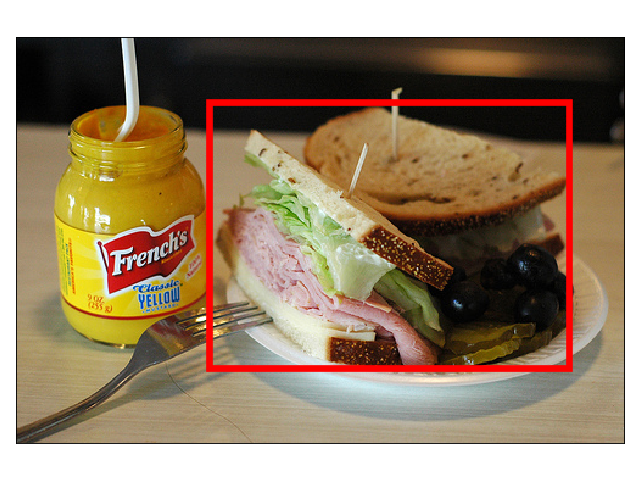
\includegraphics[width=0.9\linewidth]{figures/2339876_3928476_supercat_unique.png}} &
				\raisebox{-\totalheight}{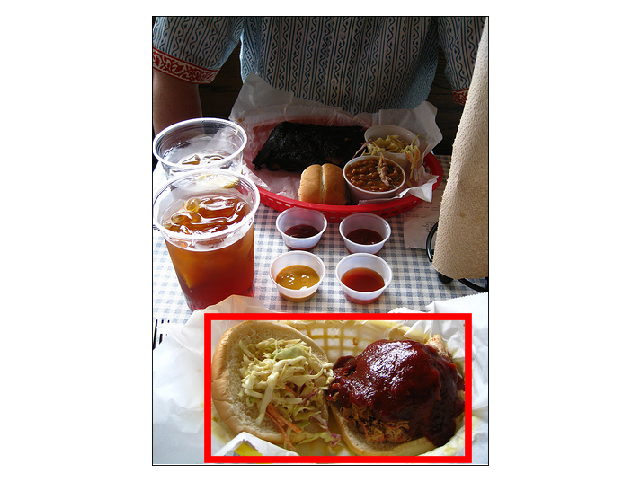
\includegraphics[width=0.9\linewidth]{figures/2379889_1353176_supercat_unique.png}} &
				\raisebox{-\totalheight}{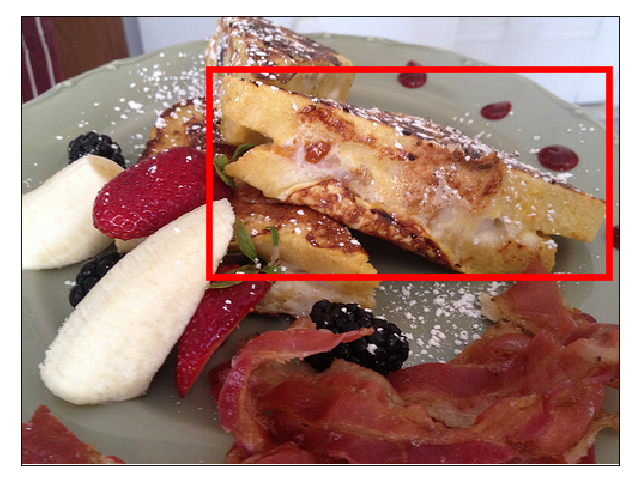
\includegraphics[width=0.9\linewidth]{figures/2394266_465678_singleton_obj.png}} &
				\raisebox{-\totalheight}{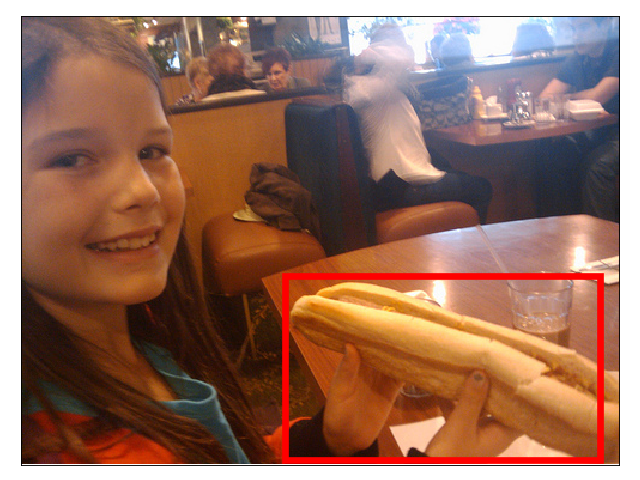
\includegraphics[width=0.9\linewidth]{figures/2386509_681763_supercat_unique.png}} \\

\textbf{A:} sandwich (34) &
\textbf{B:} sandwich (15), basket (6), food (5), burger (2),  hamburger (2),  meal (2) &
 \textbf{C:} food (10), sandwich (8), toast (5), french toast (4), dessert (2), breakfast (2) &
 \textbf{D:} hotdog (14), food (7), bun (4), sandwich (3),  bread (2)\\

        % \multicolumn{4}{c}{\textbf{VG: bridge} } \\
\raisebox{-\totalheight}{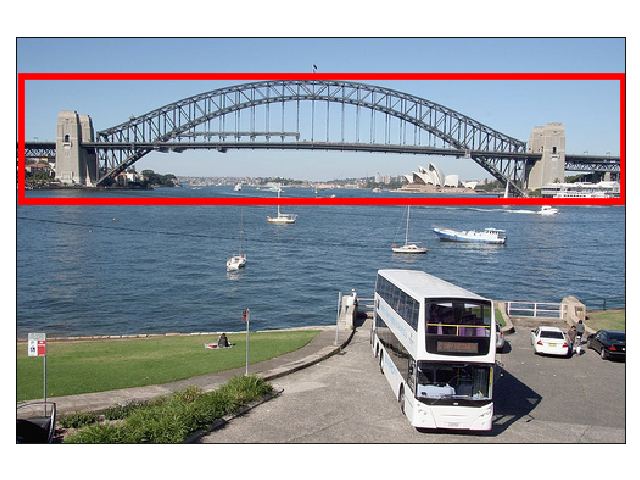
\includegraphics[width=0.9\linewidth]{figures/2341667_2006329_singleton_obj.png}} &
				\raisebox{-\totalheight}{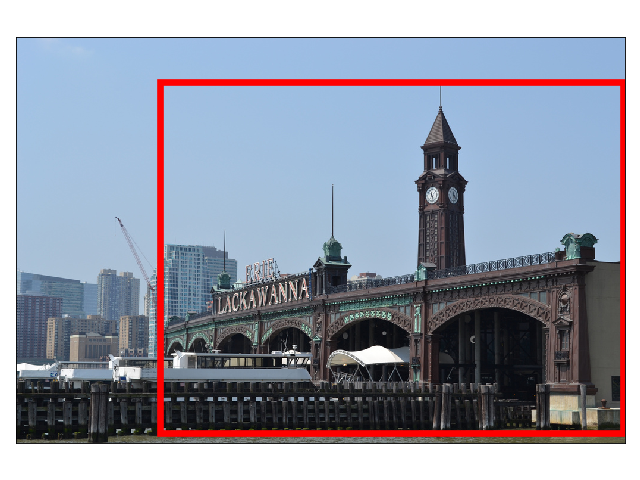
\includegraphics[width=0.9\linewidth]{figures/1592509_1610006_singleton_obj.png}} &
				\raisebox{-\totalheight}{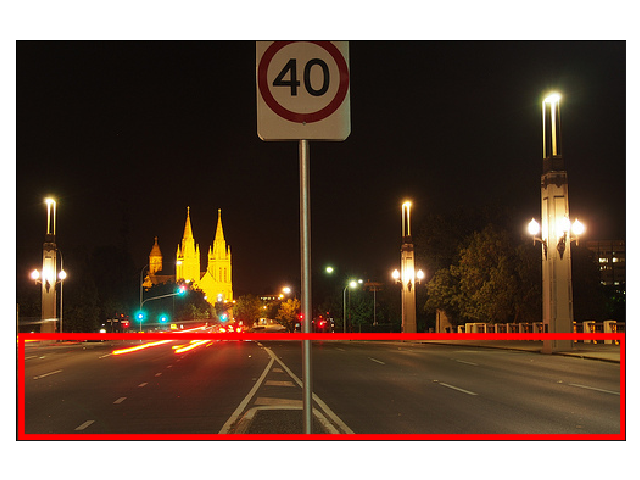
\includegraphics[width=0.9\linewidth]{figures/2384683_1306430_singleton_obj.png}} &
				\raisebox{-\totalheight}{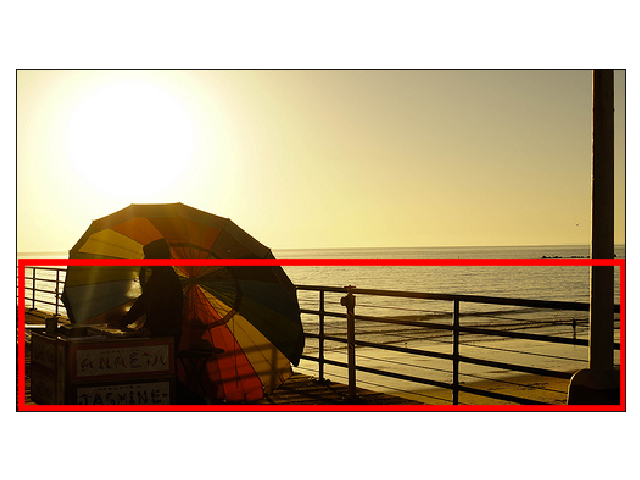
\includegraphics[width=0.9\linewidth]{figures/2412972_3494120_singleton_obj.png}} \\

 \textbf{E:} bridge (35)  &
 \textbf{F:} bridge (20),  building (11)  &
 \textbf{G:} street (16), road (15), bridge (3) &
 \textbf{H:} pier (6), railing (5), dock (5), bridge (5), fence (4), rail (3), boardwalk (3)\\
        % \multicolumn{4}{c}{\textbf{VG: bed}}\\
\raisebox{-\totalheight}{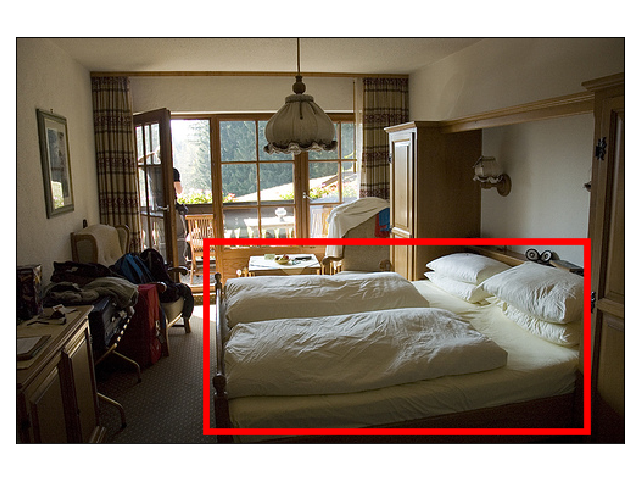
\includegraphics[width=0.9\linewidth]{figures/2321254_3438076_singleton_obj.png}} &
				\raisebox{-\totalheight}{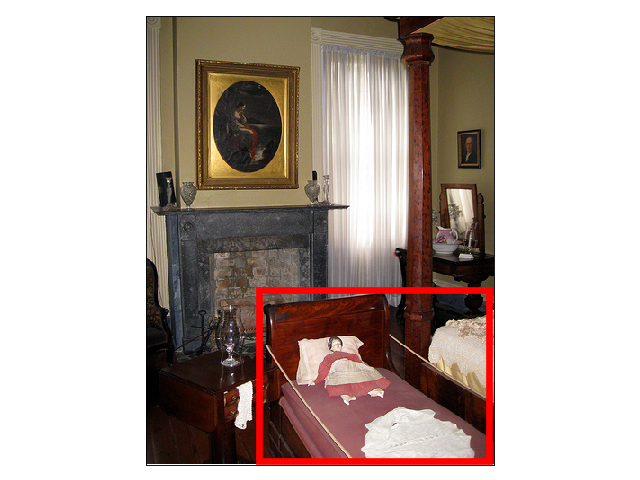
\includegraphics[width=0.9\linewidth]{figures/2324306_3412337_singleton_obj.png}} & 
				\raisebox{-\totalheight}{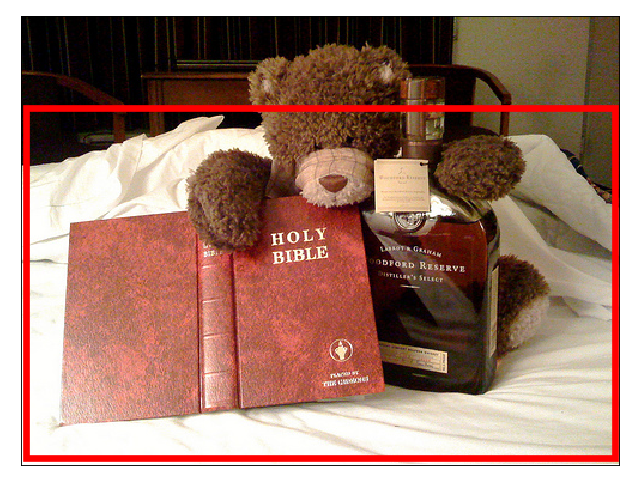
\includegraphics[width=0.9\linewidth]{figures/2342811_3485104_singleton_obj.png}} &
				\raisebox{-\totalheight}{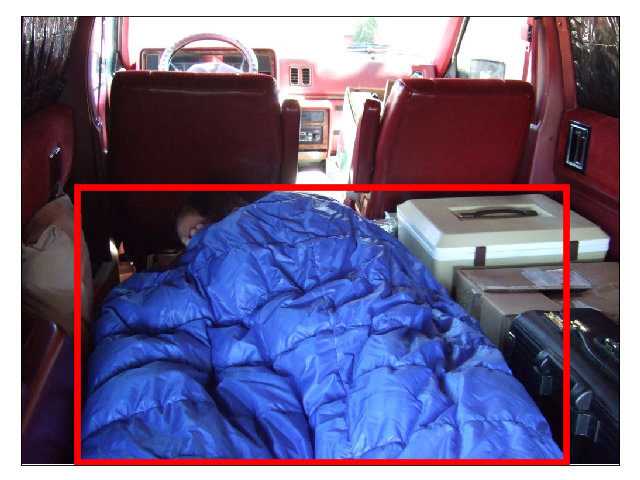
\includegraphics[width=0.9\linewidth]{figures/498222_3135415_singleton_obj.png}} \\

 \textbf{I:} bed (36)  &
 \textbf{J:} bed (16), bench (6), crib (5) &
 \textbf{K:} bed (17), book (6), table (4), toy (3), bible (2), doll (2) &
 \textbf{L:} bed (12), sleeping bag (9), blanket (7), bed sheet (5)\\

       \end{tabular}
    }
  \caption{VG images labeled \word{sandwich}, \word{bridge}, and \word{bed} (top to bottom row) with high to low agreement in ManyNames.} 
    %Names that have a hierarchical relation to the \vgenome synset in WordNet are underlined.}
	\label{fig:ex-high-low-agreement}
\end{figure*}



% \begin{figure*}[t]
%   \centering
%     {\footnotesize
%       \begin{tabular}{p{2.2cm}p{2.6cm}p{2.6cm}p{2.6cm}}
%         % \multicolumn{4}{c}{\textbf{VG: sandwich}}\\
% \raisebox{-\totalheight}{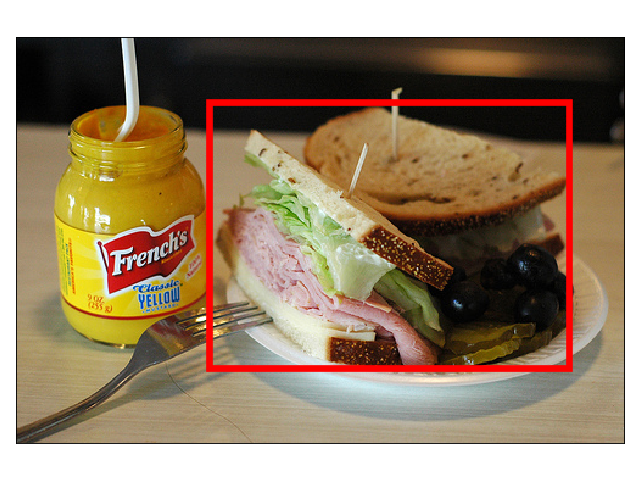
\includegraphics[width=0.9\linewidth]{figures/2339876_3928476_supercat_unique.png}} \textbf{A:} sandwich (34) &
% 				\raisebox{-\totalheight}{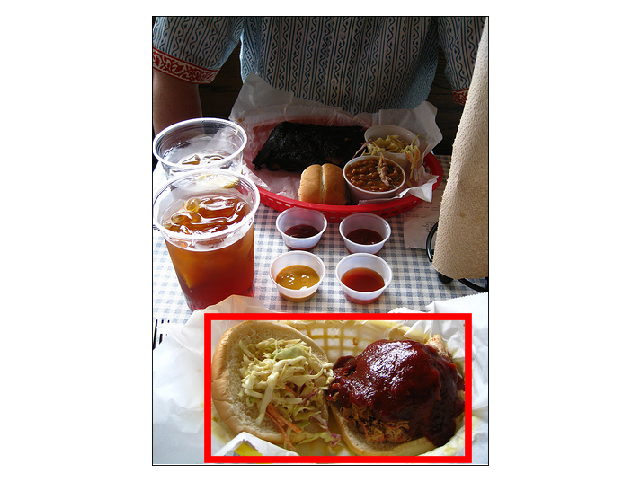
\includegraphics[width=0.9\linewidth]{figures/2379889_1353176_supercat_unique.png}} \textbf{B:} sandwich (15), basket (6), food (5), burger (2),  hamburger (2),  meal (2) &
% 				\raisebox{-\totalheight}{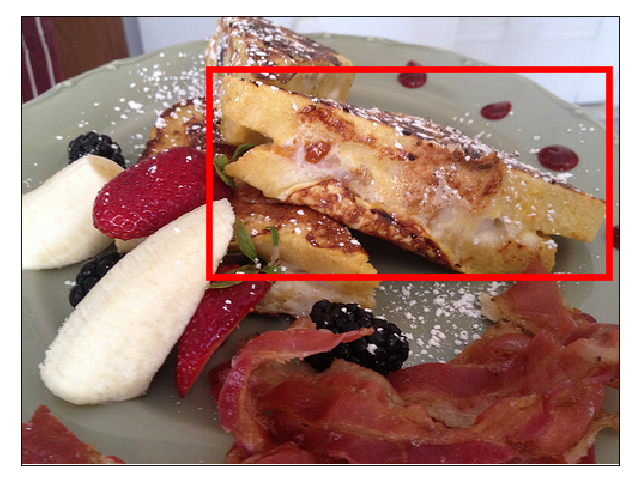
\includegraphics[width=0.9\linewidth]{figures/2394266_465678_singleton_obj.png}} \textbf{C:} food (10), sandwich (8), toast (5), french toast (4), dessert (2), breakfast (2) &
% 				\raisebox{-\totalheight}{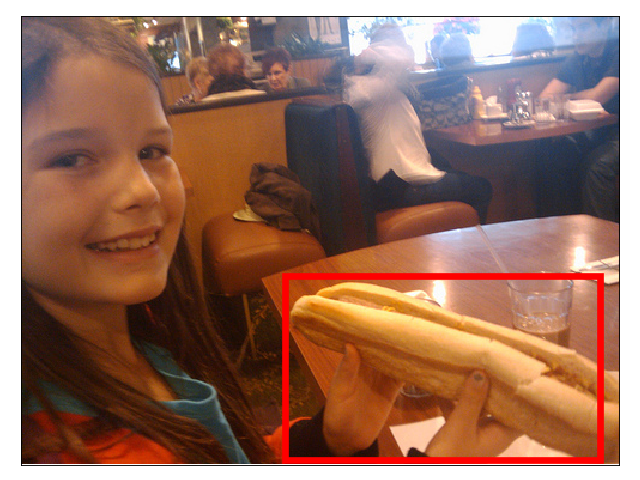
\includegraphics[width=0.9\linewidth]{figures/2386509_681763_supercat_unique.png}} \textbf{D:} hotdog (14), food (7), bun (4), sandwich (3),  bread (2) \\

%         % \multicolumn{4}{c}{\textbf{VG: bridge} } \\
% \raisebox{-\totalheight}{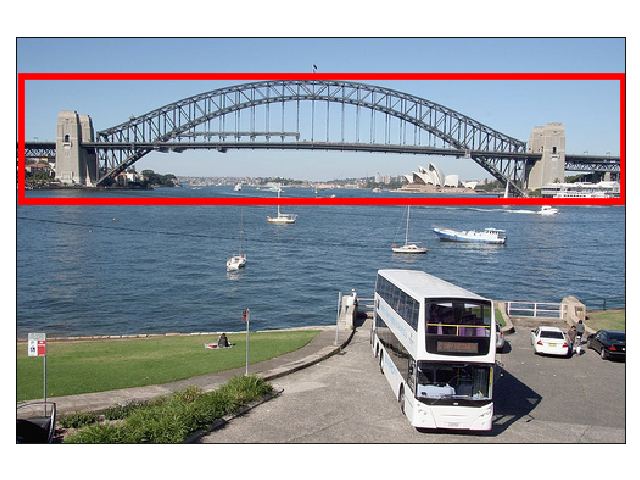
\includegraphics[width=0.9\linewidth]{figures/2341667_2006329_singleton_obj.png}} \textbf{E:} bridge (35)  &
% 				\raisebox{-\totalheight}{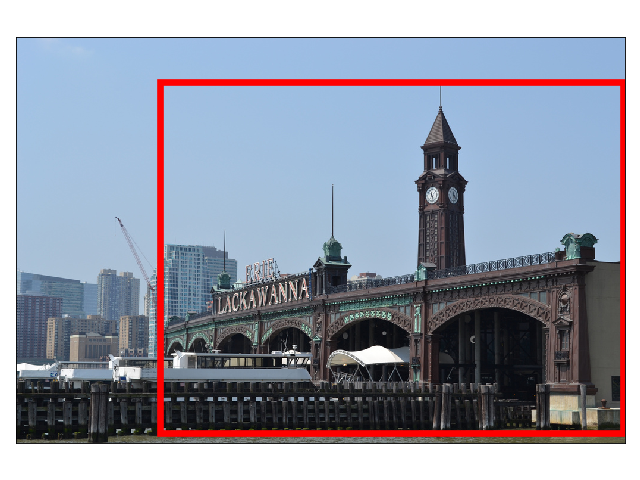
\includegraphics[width=0.9\linewidth]{figures/1592509_1610006_singleton_obj.png}} \textbf{F:} bridge (20),  building (11)  &
% 				\raisebox{-\totalheight}{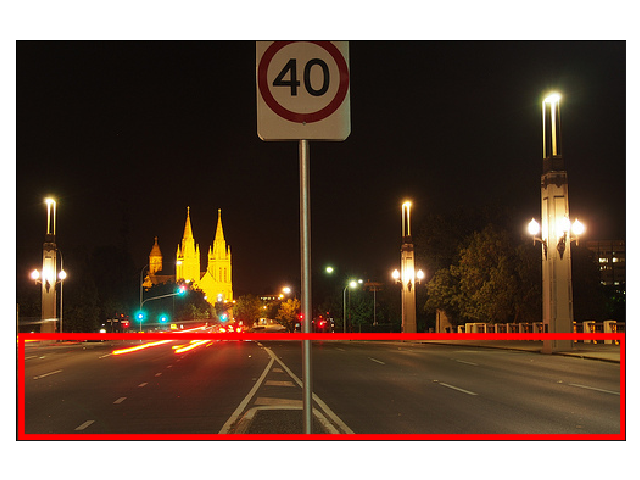
\includegraphics[width=0.9\linewidth]{figures/2384683_1306430_singleton_obj.png}} \textbf{G:} street (16), road (15), bridge (3) &
% 				\raisebox{-\totalheight}{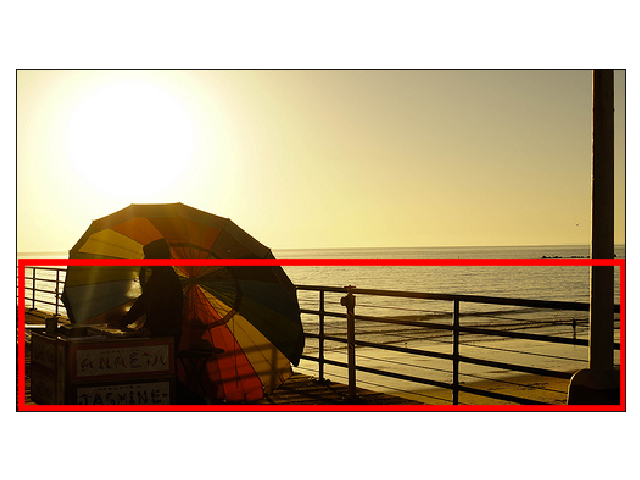
\includegraphics[width=0.9\linewidth]{figures/2412972_3494120_singleton_obj.png}} \textbf{H:} pier (6), railing (5), dock (5), bridge (5), fence (4), rail (3), boardwalk (3)\\
%         % \multicolumn{4}{c}{\textbf{VG: bed}}\\
% \raisebox{-\totalheight}{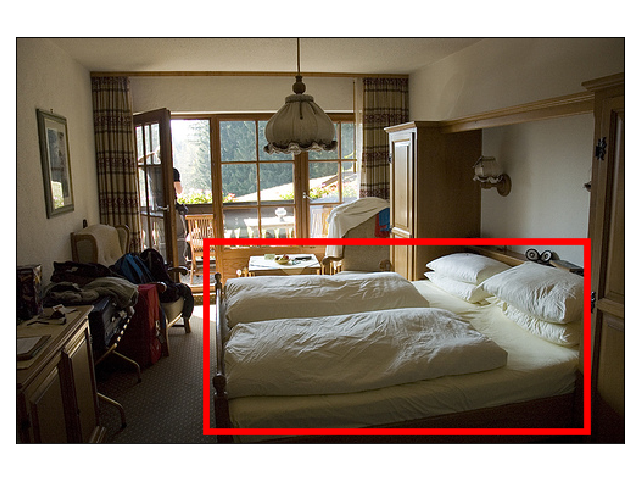
\includegraphics[width=0.9\linewidth]{figures/2321254_3438076_singleton_obj.png}} \textbf{I:} bed (36)  &
% 				\raisebox{-\totalheight}{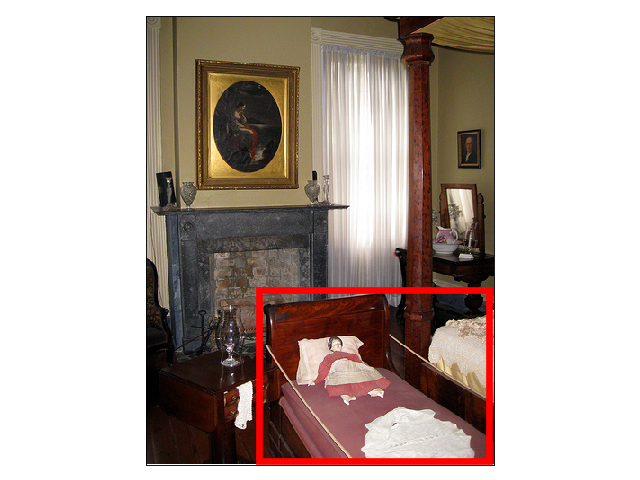
\includegraphics[width=0.9\linewidth]{figures/2324306_3412337_singleton_obj.png}} \textbf{J:} bed (16), bench (6), crib (5) &
% 				\raisebox{-\totalheight}{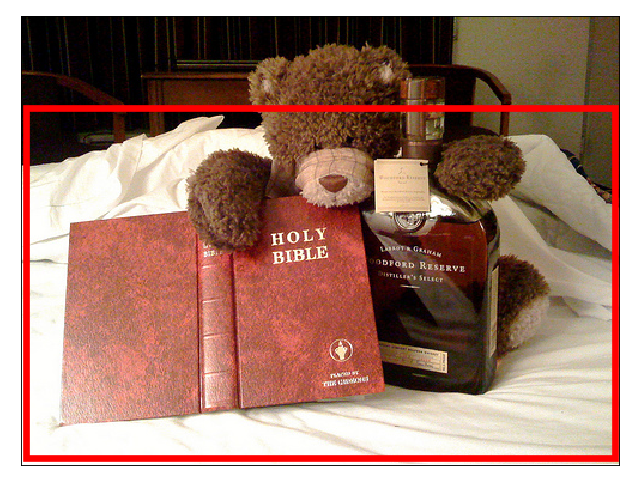
\includegraphics[width=0.9\linewidth]{figures/2342811_3485104_singleton_obj.png}} \textbf{K:} bed (17), book (6), table (4), toy (3), bible (2), doll (2) & 
% 				\raisebox{-\totalheight}{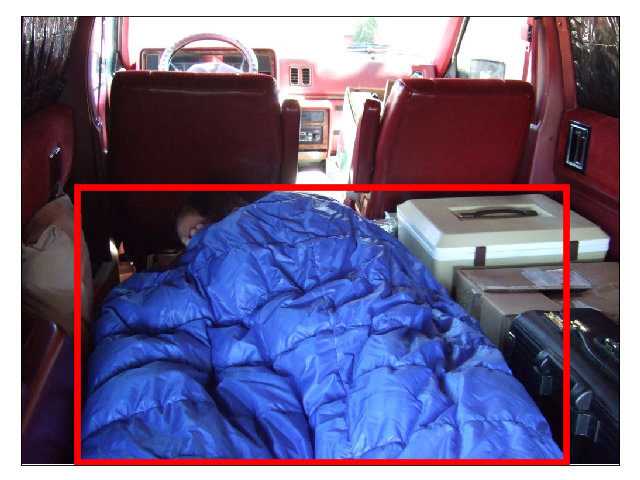
\includegraphics[width=0.9\linewidth]{figures/498222_3135415_singleton_obj.png}} \textbf{L:} bed (12), sleeping bag (9), blanket (7), bed sheet (5)\\
%       \end{tabular}
%     }
%   \caption{Examples for \vgenome images labeled \word{sandwich}, \word{bridge}, and \word{bed} (first, second, last row, respectively) with higher to lower agreement in ManyNames.} 
%     %Names that have a hierarchical relation to the \vgenome synset in WordNet are underlined.}
% 	\label{fig:ex-high-low-agreement}
% \end{figure*}



%%% Local Variables:
%%% mode: latex
%%% TeX-master: "lrec2020naming"
%%% End:


\begin{figure}
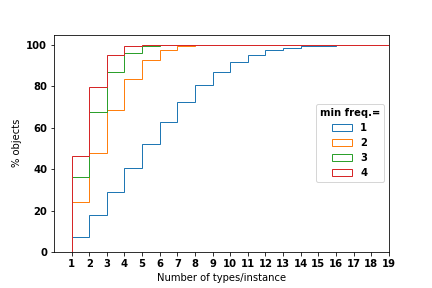
\includegraphics[width=\columnwidth]{figures/types_instances.png}
 \caption{\label{fig:ntypes} Cumulative histograms for number of types in ManyNames, with frequency thresholds} 
\end{figure}

As shown in Table~\ref{tab:compare} above, ManyNames gathers many more names per object than previous datasets: $35.3$~on average, compared to~$1-7$.
It also contains the most variability, since objects have on average $5.7$~names (compared to~\mbox{$1-1.9$}).
Figure~\ref{fig:ex-high-low-agreement} shows some example datapoints of ManyNames with high and low name agreement.
ManyNames 
%in in principle suitable to study 
shows high potential use for studying the degree of inter-subject naming agreement, and what factors influence variation.
Data analysis shows that object identification remains an issue in our data, though: Despite our care in filtering out objects that are occluded or have unclear bounding boxes (see\ Section~\ref{sec:data}), we still find many examples where annotators identified different objects for the same box. 
Typically, workers named an adjacent object or one supported by the target object (such as \word{toy/book} instead of \word{bed} in Fig.~\ref{fig:ex-high-low-agreement}, image K), or a part of the target object.
While some of these cases are arguably annotation errors, in many cases it is not possible to distinguish which object is being indicated by the  box, as in the \word{bed/sleeping bag} case in Fig.~\ref{fig:ex-high-low-agreement} (image L).
Referential uncertainty of this kind is a roadblock for the use of L\&V resources to study naming variation.
Note that pointing gestures in natural communication are as referentially uncertain as bounding boxes, if not more; however, typically those gestures are grounded in a specific discourse context, which helps to reduce uncertainty.
In future work, we plan to filter out these cases.

\subsection{Naming Variation and Agreement}
\label{subsec:counts}

We analyze the response sets obtained per object, that is, the set of names and their frequency (number of annotators entering a particular name).
Our analysis of naming variation shows that, on the one hand, we have a fair bit of consistency in the names chosen for objects, and, on the other, also consistent variation.
Figure \ref{fig:ntypes} shows the cumulative histograms for type counts, i.e.\ how many objects have at least $n$\ names, with different frequency thresholds~$t$.
Without any frequency thresholding~\mbox{$t$=1}, that is, allowing names entered by only one annotator, the proportion of instances that have a single name annotated is very small, below\ $10\%$, and there is a long tail of datapoints with many names, up to 19. 
With a reasonable (based on data inspection; names entered by one annotator only have the most noise, which is to be expected) threshold of $t$=2, a bit over $20\%$\ of the objects have one name, almost $50\%$\ up to $3$\ names, and $100\%$\ up to $8$\ names.
This threshold is the one illustrated in Fig.~\ref{fig:ex-high-low-agreement}, which shows names that have at least frequency 2.
The average number of names with this threshold is\ $2.9$, and the most frequent name accounts on average for $75\%$\ of the responses for a given object (Table~\ref{tab:agree}, and see below).
Hence, in our data, objects tend to have a preferred name, as expected from work in Psychology \cite{rosch1976basic,jolicoeur1984pictures}, but at the same time there is variation.

\begin{table}
\centering
\small
\begin{tabular}{lccccc}
  \toprule
% & \multicolumn{5}{c}{Instance-level agreement} \\
  Domain &    N &         \%top (std) &          H (std) & t=VG &   \%VG \\
  \midrule
  all &  2.9 &  75.2 (21.9) &  0.9 (0.7) &   72.8 &  62.8 \\
  \midrule
  people &  4.3 &  59.0 (20.4) &  1.5 (0.7) &   49.8 &  36.3 \\
  clothing &  3.2 &  70.1 (18.5) &  1.1 (0.6) &   70.2 &  57.4\\
  home &  3.1 &  72.6 (20.7) &  1.0 (0.7) &   78.5 &  64.1 \\
  buildings &  3.0 &  74.7 (20.7) &  1.0 (0.7) &   72.6 &  61.6\\
  food &  2.9 &  76.4 (20.7) &  0.9 (0.7) &   62.9 &  55.2 \\
  vehicles &  2.4 &  76.6 (19.8) &  0.8 (0.6) &   71.1 &  63.9 \\
  animal\_plants &  1.5 &  94.5 (12.1) &  0.2 (0.4) &   93.8 &  91.0\\
\bottomrule
\end{tabular}
\vspace{-0.3cm}
\caption{Agreement in object naming, with a frequency threshold of~$2$.}
% Domain `an\_pl' is animal\_plants.}
\label{tab:agree}
\end{table}

To further assess agreement on the object names, we check the following measures, computed with \mbox{$t$=$2$}, with results in Table~\ref{tab:agree}:
\begin{itemize}
\item \textbf{N}: the average number of types in the response set. %of ManyNames.
\item \textbf{\% top}: the average relative frequency of the most frequent response (shown in percent).
\item $\mathbf{H}$: the $H$ agreement measure from \cite{snodgrass}, where $0$~is perfect agreement: \mbox{$H = \sum_{i=1}^k p_i~log_2\frac{1}{p_i}$}, 
where $k$~denotes the number of name types and $p_i$~is the proportion of type~$i$ in the responses. 
\item \textbf{t=VG}: the percentage of items where the top response in ManyNames is the \vg name.
\item \textbf{\% VG}: the average relative frequency of the \vg name in the response set.
\end{itemize}

Apart from the trends mentioned above, it is remarkable that only in $73$\%~of the cases the most frequent response coincides with the \vg name, and the \vg name accounts for $63$\%~of the responses on average.
Our dataset can be expected to yield a more robust estimate for so-called entry-point names \cite{jolicoeur1984pictures}, that is, the name that most naturally comes to mind for a given object.
The $H$ measures indicate a fair amount of agreement, a bit lower than in picture norming studies on artificial idealized images (e.g.\ \newcite{snodgrass} report an average $H$ of~$0.55$), which can be expected when using real images.

If we check agreement by domain, two domains stand out: the \domain{animals\_plants} domain, which is often discussed in the literature and where we find almost perfect agreement\ (\mbox{$H=0.2$}), and the \domain{people} domain with a particularly low agreement.
Across domains, however, we find a large standard deviation for both \%top and $H$, of around\ $20\%$ for all domains except \domain{people}.
This indicates that agreement varies quite a bit across instances, with factors that cannot be attributed to domain only.
The qualitative examples in Figure \ref{fig:ex-high-low-agreement} illustrate this, showing instances with very high or low agreement.
These suggest that instances which are more prototypical of a category trigger higher agreement, although further research is necessary to examine the relevant factors.
The following section will examine other sources of variation in object naming.

%\begin{table}
%\small
%\begin{tabular}{lp{4.8cm}r}
%\toprule
%VG name &  top5 MN names &  n$_{obj}$  \\
%\midrule
%\multicolumn{3}{c}{\it Canonical VG names with max agreement in MN}\\
% giraffe &  giraffe (96.8), animal (1.2), zebra (0.4), camel (0.3), pole (0.1) &  915 \\
% zebra &  zebra (96.3), animal (1.0), giraffe (0.9), horse (0.2), microwave (0.2) &  461  \\
% cat &  cat (94.8), animal (0.9), kitten (0.8), dog (0.4), laptop (0.2) &  754\\
%\midrule
%\multicolumn{3}{c}{\it Canonical VG names with min agreement in MN}\\
% booth &  booth (19.3), table (12.3), phone booth (9.8), bench (6.7), building (4.4) &  11 \\
% cabbage &  cabbage (21.4), lettuce (17.0), hotdog (11.9), food (10.7), salad (10.4) &  9 \\
% robe &  robe (22.1), shirt (16.8), jacket (13.3), dress (5.7), clothing (3.2) &  19 \\
%  \midrule
%  \multicolumn{3}{c}{\it Non-canon. VG names with max agreement in MN}\\
% sedan &  car (88.4), wheel (3.1), vehicle (2.3), automobile (1.3), dog (0.8) &  11 \\
% pony &  horse (83.9), pony (9.1), animal (2.9), donkey (1.1), cow (1.1) &  8 \\
% necktie &  tie (81.4), necktie (10.2), shirt (4.6), ties (1.5), jacket (0.5) &  11 \\
% \midrule
%   \multicolumn{3}{c}{\it Non-canon. VG names with min agreement in MN}\\
% shelter &  umbrella (9.7), shelter (8.8), roof (8.0), tent (7.1), building (6.8) &  10 \\
% bath &  shower (13.3), elephant (9.9), birdbath (8.1), water (7.2), trough (7.2) &  10 \\
% vegetable &  food (15.7), broccoli (13.1), sandwich (10.6), salad (9.3), pizza (7.8) &  25 \\
%\bottomrule
%\end{tabular}
%\caption{Examples for VisualGenome (VG) names and their most frequent corresponding responses in ManyNames (MN; percentages shown in brackets). ``Canonical'' means that the VG name is the top name in MN, and non-canonical vice versa.}
%\label{tab:qual}
%\end{table}

%\gbt{The non-canon. VG names suggest that people prefer more general names (``car $>$ sedan'', ``horse $>$ pony'', ``tie $>$ necktie''). Could be due to lexical availability (more general \ra more frequent \ra more available). This could be verified (using frequency). Hypothesis: In cases where top name != VG, the VG name is less general. Could be also a more general hypothesis: see if people prefer more frequent names in general.}
%\cs{@Table~\ref{tab:qual} (just wrt presentation) The most interesting blocks are 2 and 3 (canonical VG with min agr.; non-canonical with max agr.)}

\subsection{Sources of Variation}
\label{subsec:sources}

Previous work on object naming has assumed that variation is mostly along a taxonomic axis, and in particular hierarchical (see Section~\ref{sec:rel-work}).
This parameter does not seem to explain the variation in ManyNames. 
Table \ref{tab:rel} shows the distribution of the lexical relations between ManyNames responses and the original \vg annotation, estimated from WordNet.
To obtain these data, we exploited the synset annotation in the \vg names, and added automatic linking for the additional ManyNames names, with a simple first-sense heuristic.%
\footnote{To detect hypernyms, we use the hypernym closure of the synset with a depth of $10$; the other relations are straightforward. The coverage of WordNet for our name data is satisfactory ($90$\%\ of the name types, accounting for $97$\%\ of the tokens).}
As shown in the table, in the vast majority of cases, no hierarchical relation between the name and the synset can be retrieved from WordNet.
Even factoring in the noise introduced by referential uncertainty, it is clear that a good portion of our data cannot be explained by variation in the level of abstraction of the chosen name. 
Among the names that do have a taxonomic relation to the synset, hypernyms are the most frequent, meaning that our annotators often went for a more general name than the \vg annotators.
%%In this section, we take a closer look at the lexical variation we observe in our data set. 
%We analyze the data points where participants attributed different names to the same object and extract a set of  pairwise \textbf{naming variants}. These naming variants correspond to pairs of words that can be used interchangeably to name certain objects.
%For each object, we extract the set of naming variants $s = \{ (w_{top},w_2), (w_{top},w_3), (w_{top},w_4),... \}$  where $w_{top}$ is the most frequent name annotated for the object and $w_2 ... w_n$ constitute the less frequent alternatives of $w_{top}$.  The  \textbf{type frequency} of a naming variant $(w_{top},w_x)$ corresponds to the number of objects where this variant occurs. The \textbf{token frequency} of $(w_{top},w_x)$ corresponds the count of all annotations where $w_x$ has been used instead of $w_{top}$.
%In Table \ref{tab:exvariants}, we show the naming variants with the highest raw token frequency for each domain. 
%The naming variants can be grouped according to their lexical relation, as follows:
%
%\begin{itemize}
%\item \textbf{synonymy}: e.g.\ aircraft vs. airplane 
%\item \textbf{hyponymy}: e.g.\ man vs. person
%\item \textbf{co-hyponymy}: e.g.\ swan vs. goose
%\item \textbf{no relation}: e.g.\  desk vs. apple
%\end{itemize}
%\cs{Shouldn't we mention that we consider only simple move-up hypernymy relations?}

%and the VG synsets) in the aggregated class-level response sets." // "Table \ref{tab:rel} shows the relative frequency distribution of the different relations which occur between the MN names and the VG synsets in the aggregated class-level response sets."} 
%\gbt{what do you mean, `` aggregated class-level response set''?}
%\cs{Considering the track we are submitting to, one or two examples per relation in an additional column in the table wouldn't hurt.}

In a qualitative analysis, we found the following types of variation in the data, illustrated with examples in Figure~\ref{fig:ex-high-low-agreement}.
\textbf{Cross-classification}: a substantial group are names conceptualizing alternative aspects of the same object (e.g. \word{toast/dessert}, image C).
\textbf{Conceptual disagreement}: as we did not filter objects for prototypicality, our data mirrors a certain amount of disagreement between speakers as to what an object is (\word{bed/bench}, images J).
\textbf{Metonymy}: we find examples reminiscent of metonymy discussed in the linguistic literature \cite{pustejovsky1991generative} where logically related parts of an object stand in as its name (\word{burger/basket}, image B). 
\textbf{Issues with WordNet}: due to WordNet's fine-grained hierarchy, it is difficult to retrieve certain loose synonyms or hypernyms (\word{robe/dress}, image not shown).
%As it is non-trivial to separate these phenomena, we leave a quantitative analysis for future work.
%
\cs{TO ADD: What does ManyNames provide, that WordNet can't: out-of-vocabulary words; we observe instance-based variation, WordNet is class-based: valid (co-)hyponyms, different most preferred name depending on instance, variations which are not due to taxonomic relations}
\begin{table}[t]
%\small
\centering
\setlength{\tabcolsep}{2pt}
\begin{tabular}{lcc|p{2.5cm}}
\toprule
         relation & \% types & \% tokens & \it ex: jacket \\
\midrule
% meronym &  0.1 &  0.2 \\
% holonym &  0.1 &  0.4 \\
 word-not-covered &  10.6 &  2.6 & \it outdoor vest\\
\midrule
 synonym &  1.1 &  1.1 & \it hoodie  \\
 hyponym &  2.2 &  3.8 & \it parka\\ %, blazer \\
 co-hyponym &  3.1 &  5.9 & \it raincoat\\
 hypernym &  10.5 &  27.7 & \it clothing \\%, coat\\
 rel-not-covered &  72.2 &  58.3 & \it sweatshirt\\%, man\\
\bottomrule
\end{tabular}
\caption{Lexical relations of naming variants in ManyNames to annotated \vg synset, averaged over synsets, with examples of variants for \word{jacket}.}
\label{tab:rel}
\vspace{-0.5cm}
\end{table}


\iffalse
*********
Existing large-scale collections of labels or names of objects in L\&V provide simple annotations of individual objects with canonicalized name sets.
When humans agree only around 70\% of the cases in how to name an object, it is not clear that the data can be taken as a gold standard in multi-label classification setting, as is commonly done in Computer Vision.
% At the same time, compared to annotation and modeling frameworks in Computer Vision that frame the problem as an object labeling task, our data shows a much lower agreement than what should be expected if object names were indeed entirely canonical,
See e.g.\ the ResNet which achieves a top-1 error rate of $25$\% on ILSVRC 2015. \gbt{It is not clear to me what this means: what kind of data is this? how does this result relate to our point? -- @Carina, expand?}
\fi

%\gbt{I couldn't follow the discussion in the following pargraph. Do you think it's subsumed by the one above? Can we remove it?} 
%Given that we find much lower agreement on object class-level than on an instance-level, one might argue for using very fine-grained object annotations to remedy this problem. 
%However, the fact that naming variants are often not recoverable by hierarchical relations suggest that even fine-grained recognition models cannot be expected to be able to simply infer recognition of more general classes (e.g., ILSVRC synset). Thus, neither simple multi-label classification nor more advance hierarchical approaches to object recognition seem to be well designed for capturing natural naming phenomena comprising cross-classification, metonymy and potentially other sources of variation.

%What does this discrepancy between the instance-level and category-level agreement in VisualGenome and ManyNames naming choices mean? 
%First of all, it suggests that the same original VisualGenome name can trigger very different variants depending on the visual instance, leading to a drastic increase of variants elicited for categories as compared to instances.
%Second, this clearly shows that annotators in VG do not generally annotate the most canonical name \cs{but they don't annotate the name, but the description} and that many names annotated for objects in VG do not correspond to the overall most preferred variant. \sz{think more ...}
%\gbt{I don't think we can conclude this second part -- we do have the 70\% top=VG figure that says that VG annotators annotate the most canonical name. What this suggests to me is that instance-level properties are more important than category-level properties, somehow.

%Why is naming more flexible in certain domains than in others? \gbt{Hypothesis: expectation: little variation - hypernymy at most, more variation <-> more affordances <-> more varied relationships.}

%\cs{@Table~\ref{tab:agree} I still think that we could also have \%\ top with $N>1$ to give an idea as to how useful the data is for the people interested in using it for, e.g., model evaluation. For that, it is clear that crowdsourcing is noisy and before using it some outlier removal needs to be made.}

% \subsection{Entry-level names and preference orders....}

% \sz{an interesting example:} In our data set, there are 24 images where \textit{penguin} has been used, so we know that the object is a \textit{penguin}. For 50\% of these images, annotators still prefer \textit{bird} as the most common name. According to the theory of entry-level categories, this should not happen. People should always prefer \textit{penguin} over \textit{bird}. 

% \sz{how can we analyze this quantitatively?}

% \begin{itemize}
% \item lettuce -- salad
% \item fruit -- food
% \item man -- catcher
% \item bowl --chili
% \item bowl -- diner \gbt{spelling mistake? should be dinner?} 
% \item burger -- meat
% \item statue -- animal (image shows statue of an animal)
% \item bottle -- alcohol
% \item donut --desert \gbt{spelling mistake? should be dessert?} 
% \item zebra -- stripes
% \item oven -- grill
% \end{itemize}


%%% Local Variables:
%%% mode: latex
%%% TeX-master: "lrec2020naming"
%%% End:


